\chapter{Specifikacija programske potpore}
		
	\section{Funkcionalni zahtjevi}
			
			
			\noindent \textbf{Dionici:}
			
			\begin{packed_enum}
				
				\item Vlasnik kućnog ljubimca
				\item Sklonište za životinje			
				\item Ostali korisinici aplikacije(klijent)
                \item Razvojni tim
				
			\end{packed_enum}
			
			\noindent \textbf{Aktori i njihovi funkcionalni zahtjevi:}
			
			
			\begin{packed_enum}
				\item  \underbar{Neregistrirani korisnik (inicijator) može:}
				
				\begin{packed_enum}
					
					\item pretraživati oglašene nestale kućne ljubimce i skloništa za životinje
					\item detaljno pregledavati informacije o nestalim kućnim ljubimcima
					\item  pregledavati komunikaciju oko potrage za ljubimcem
					
				\end{packed_enum}

                \item  \underbar{Vlasnik kućnog ljubimca (inicijator) može:}
				
				\begin{packed_enum}
					
					\item postaviti oglas o nestalom kućnom ljubimcu
					\item sudjelovati u komunikaciji oko potrage za ljubimcem
					\item ukloniti oglas o nestalom kućnom ljubimcu
					\item izmijeniti oglas o nestalom kućnom ljubimcu
					\item pretraživati neaktivne oglase o nestalim kućnim ljubimcima
					\item sve što i neregistrirani korisnik može
					
				\end{packed_enum}

                \item  \underbar{Sklonište za životinje (inicijator) može:}
				
				\begin{packed_enum}
					
					\item oglašavati životinje koje je pronašlo i koje se nalazi u njegovom prostoru
					\item postaviti posebnu kategoriju ("u skloništu") kod postave oglasa
					\item sve što i vlasnik kućnog ljubimca može
					
				\end{packed_enum}
			
				\item  \underbar{Baza podataka (sudionik):}
				
				\begin{packed_enum}
					
					\item pohranjuje sve podatke o registriranim korisnicima, njihovim oglasima i komunikacijama oko potrage za ljubimcem
					\item pohranjuje sve podatke o skloništima za životinje, njihovim oglasima i komunikacijama oko potrage za ljubimcem
					
				\end{packed_enum}
			\end{packed_enum}
			
			\eject 
			
			
				
			\subsection{Obrasci uporabe}
				
				\subsubsection{Opis obrazaca uporabe}		

					\noindent \underbar{\textbf{UC1 - Pregled oglasa nestalih ljubimaca}}
					\begin{packed_item}
	
						\item \textbf{Glavni sudionik: }Neregistrirani korisnik, Vlasnik kućnog ljubimca, Sklonište za životinje
						\item  \textbf{Cilj:} Pregledavanje oglašenih nestalih kućnih ljubimaca i skloništa za životinje
						\item  \textbf{Sudionici:} Baza podataka
						\item  \textbf{Preduvjet:} -
						\item  \textbf{Opis osnovnog tijeka:}
						
						\item[] \begin{packed_enum}
	
							\item Nestali ljubimci su prikazani prilikom učitavanja aplikacije
							\item Korisnik odabire nestalog ljubimca
							\item Prikazuje se detaljniji pregled informacija i pregled komunikacija oko potrage
						\end{packed_enum}
						
					\end{packed_item}
				
					\noindent \underbar{\textbf{UC2 - Registracija}}
					\begin{packed_item}
						
						\item \textbf{Glavni sudionik: }Neregistrirani korisnik 
						\item  \textbf{Cilj:} Stvoriti korisnički račun za pristup sustavu
						\item  \textbf{Sudionici:} Baza podataka
						\item  \textbf{Preduvjet:} -
						\item  \textbf{Opis osnovnog tijeka:}
						
						\item[] \begin{packed_enum}
							
							\item Korisnik odabire opciju za registraciju
							\item Korisnik unosi vlastite podatke
							\item Podaci se spremaju u bazu podataka
							\item Korisnik prima obavijest o uspješnoj registraciji
						\end{packed_enum}
						
						\item  \textbf{Opis mogućih odstupanja:}
						
						\item[] \begin{packed_item}
							
							\item[2.a] Podaci koje je korisnik unio odgovaraju postojećem korisničkom računu
							\item[] \begin{packed_enum}
								
								\item Pojavljuje se poruka o neuspješnoj registraciji i zahtjev za ponovnim unosom podataka
								\item Korisnik mijenja podatke ili odustaje od registracije
								
							\end{packed_enum}
							\item[2.b] Korisnik nije unio sve zahtijevane podatke
								\item[] \begin{packed_enum}
								
								\item Pojavljuje se poruka o neuspješnoj registraciji i zahtjev za ponovnim unosom podataka
								\item Korisnik unosi zahtijevane podatke ili odustaje od registracije
								
							\end{packed_enum}
							
						\end{packed_item}
					\end{packed_item}
					
					\noindent \underbar{\textbf{UC3 - Pretraživanje oglasa nestalih ljubimaca}}
					\begin{packed_item}
						
						\item \textbf{Glavni sudionik: }Neregistrirani korisnik, Vlasnik kućnog ljubimca, Sklonište za životinje
						\item  \textbf{Cilj:} Pretraživanje nestalih ljubimaca po svim dostupnim kategorijama podataka
						\item  \textbf{Sudionici:} Baza podataka
						\item  \textbf{Preduvjet:} -
						\item  \textbf{Opis osnovnog tijeka:}
						
						\item[] \begin{packed_enum}
							
							\item Korisnik odabire kategorije podataka po kojima obavlja pretraživanje
							\item Korisnik unosi podatke (filtre) za odabrane kategorije
							\item Prikazuje se popis filtriranih oglasa
						\end{packed_enum}
					\end{packed_item}
					
					\noindent \underbar{\textbf{UC4 - Prijava u sustav}}
					\begin{packed_item}
						
						\item \textbf{Glavni sudionik: }Vlasnik kućnog ljubimca, Sklonište za životinje
						\item  \textbf{Cilj:} Dobiti pristup korisničkom sučelju
						\item  \textbf{Sudionici:} Baza podataka
						\item  \textbf{Preduvjet:} Registracija
						\item  \textbf{Opis osnovnog tijeka:}
						
						\item[] \begin{packed_enum}
							
							\item Unos korisničkog imena ili e-mail adrese i lozinke
							\item Provjera ispravnosti unesenih podataka
							\item Pristup korisničkom sučelju web aplikacije
						\end{packed_enum}
						
						\item  \textbf{Opis mogućih odstupanja:}
						
						\item[] \begin{packed_item}
							
							\item[2.a] Korisnik je unio nepostojeće korisničko ime ili e-mail adresu
							\item[] \begin{packed_enum}
								
								\item Pojavljuje se poruka o neuspješnoj prijavi i zahtjev za ponovnim unosom podataka
								\item Korisnik unosi ispravne podatke ili odustaje od prijave
								
							\end{packed_enum}
							\item[2.b] Korisnik je unio neispravnu lozinku za odgovarajuće korisničko ime odnosno e-mail
							\item[] \begin{packed_enum}
								
								\item Pojavljuje se poruka o neuspješnoj prijavi i zahtjev za ponovnim unosom podataka
								\item Korisnik unosi ispravne podatke ili odustaje od prijave
								
							\end{packed_enum}
							
						\end{packed_item}
					\end{packed_item}
					\pagebreak
					\noindent \underbar{\textbf{UC5 - Komuniciranje oko potrage za nestalim ljubimcem}}
					\begin{packed_item}
						
						\item \textbf{Glavni sudionik: }Vlasnik kućnog ljubimca, Sklonište za životinje
						\item  \textbf{Cilj:} Ostvariti komunikaciju s vlasnikom izgubljenog ljubimca
						\item  \textbf{Sudionici:} Baza podataka
						\item  \textbf{Preduvjet:} Korisnik je prijavljen
						\item  \textbf{Opis osnovnog tijeka:}
						
						\item[] \begin{packed_enum}
							
							\item Korisnik odabire nestalog ljubimca
							\item Prikazuje se popis komunikacije oko potrage za ljubimcem
							\item Korisnik unosi poruku koja može sadržavati tekst, sliku i geolokaciju
						\end{packed_enum}
					\end{packed_item}
					
					\noindent \underbar{\textbf{UC6.1 - Postavljanje oglasa nestalog ljubimca}}
					\begin{packed_item}
						
						\item \textbf{Glavni sudionik: }Vlasnik kućnog ljubimca, Sklonište za životinje
						\item  \textbf{Cilj:} Postaviti oglas o izgubljenom ljubimcu
						\item  \textbf{Sudionici:} Baza podataka
						\item  \textbf{Preduvjet:} Korisnik je prijavljen
						\item  \textbf{Opis osnovnog tijeka:}
						
						\item[] \begin{packed_enum}
							
							\item Korisnik odabire opciju za novi oglas
							\item Korisnik unosi podatke o ljubimcu za zadane kategorije
							\item Korisnik objavljuje oglas
						\end{packed_enum}
						
						\item  \textbf{Opis mogućih odstupanja:}
						
						\item[] \begin{packed_item}
							
							\item[2.a] Korisnik je unio invalidne podatke u određenu kategoriju
							\item[] \begin{packed_enum}
								
								\item Pojavljuje se poruka o pogrešci i zahtjev za ponovnim unosom podataka
								\item Korisnik unosi ispravne podatke ili odustaje od objave oglasa
								
							\end{packed_enum}
							\item[2.b] Korisnik nije unio potrebne podatke
							\item[] \begin{packed_enum}
								
								\item Pojavljuje se poruka o pogrešci i zahtjev za ponovnim unosom podataka
								\item Korisnik unosi zahtijevane podatke ili odustaje od objave oglasa
								
							\end{packed_enum}
						\end{packed_item}
					\end{packed_item}
					\pagebreak
					\noindent \underbar{\textbf{UC6.2 - Uklanjanje oglasa nestalog ljubimca}}
					\begin{packed_item}
						
						\item \textbf{Glavni sudionik: }Vlasnik kućnog ljubimca, Sklonište za životinje
						\item  \textbf{Cilj:} Ukloniti oglas o izgubljenom ljubimcu
						\item  \textbf{Sudionici:} Baza podataka
						\item  \textbf{Preduvjet:} Korisnik je prijavljen i objavio je oglas
						\item  \textbf{Opis osnovnog tijeka:}
						
						\item[] \begin{packed_enum}
							
							\item Korisnik odabire oglas
							\item Korisnik odabire opciju za brisanje oglasa
							\item Oglas i sva komunikacija vezana uz njega nestaju iz popisa vidljivih oglasa
							\item Oglas ostaje pohranjen u bazi podataka
						\end{packed_enum}
						
					\end{packed_item}
					
					\noindent \underbar{\textbf{UC6.3 - Izmjena oglasa nestalog ljubimca}}
					\begin{packed_item}
						
						\item \textbf{Glavni sudionik: }Vlasnik kućnog ljubimca, Sklonište za životinje
						\item  \textbf{Cilj:} Izmjena oglasa o izgubljenom ljubimcu
						\item  \textbf{Sudionici:} Baza podataka
						\item  \textbf{Preduvjet:} Korisnik je prijavljen i objavio je oglas
						\item  \textbf{Opis osnovnog tijeka:}
						
						\item[] \begin{packed_enum}
							
							\item Korisnik odabire opciju za izmjenu oglasa
							\item 
								\begin{packed_item}
									\item[a$)$] Korisnik mijenja podatke po kategorijama oglasa
									\item[b$)$] Korisnik mijenja kategoriju oglasa 
								\end{packed_item}
							\item Korisnik sprema promjene
						\end{packed_enum}
						
						\item  \textbf{Opis mogućih odstupanja:}
						
						\item[] \begin{packed_item}
							
							\item[2.a] Korisnik je unio invalidne podatke u određenu kategoriju
							\item[] \begin{packed_enum}
								
								\item  Pojavljuje se poruka o pogrešci i zahtjev za ponovnim unosom
								\item Korisnik unosi ispravne podatke ili odustaje od izmjene oglasa
								
							\end{packed_enum}
							\item[2.b] Korisnik je promijenio kategoriju oglasa u kategoriju koja ne odgovara aktivnoj potrazi za ljubimcem
							\begin{packed_enum}
								
								\item Oglas se prebacuje u popis neaktivnih oglasa
								
							\end{packed_enum}
							
						\end{packed_item}
					\end{packed_item}
					\pagebreak
                    \noindent \underbar{\textbf{UC7 - Odjava iz sustava}}
					\begin{packed_item}
						
						\item \textbf{Glavni sudionik: }Vlasnik kućnog ljubimca, Sklonište za životinje
						\item  \textbf{Cilj:} Odjaviti svoj korisnički profil iz aplikacije.
						\item  \textbf{Sudionici:} Baza podataka
						\item  \textbf{Preduvjet:} Korisnik je prijavljen
						\item  \textbf{Opis osnovnog tijeka:}
						
						\item[] \begin{packed_enum}
							
							\item Korisnik odabire opciju za odjavu iz sustava
							\item Korisnik se preusmjerava na sučelje neregistriranog korisnika.
						\end{packed_enum}
					\end{packed_item}
     
					\noindent \underbar{\textbf{UC8 - Oglašavanje pronađenih životinja}}
					\begin{packed_item}
						
						\item \textbf{Glavni sudionik: }Sklonište za životinje
						\item  \textbf{Cilj:} Oglašavanje pronađenih životinja koje se nalaze u prostoru skloništa
						\item  \textbf{Sudionici:} Baza podataka
						\item  \textbf{Preduvjet:} Korisnik je prijavljen
						\item  \textbf{Opis osnovnog tijeka:}
						
						\item[] \begin{packed_enum}
							
							\item Korisnik odabire opciju za novi oglas
							\item Korisnik unosi podatke o ljubimcu za zadane kategorije (uključujući i dodatnu kategoriju – u skloništu)
							\item Korisnik objavljuje oglas
						\end{packed_enum}
						
						\item  \textbf{Opis mogućih odstupanja:}
						
						\item[] \begin{packed_item}
							
							\item[2.a] Korisnik je unio invalidne podatke u određenu kategoriju
							\item[] \begin{packed_enum}
								
								\item Pojavljuje se poruka o pogrešci i zahtjev za ponovnim unosom podataka
								\item Korisnik unosi ispravne podatke ili odustaje od objave oglasa
								
							\end{packed_enum}
							\item[2.b] Korisnik nije unio potrebne podatke
							\item[] \begin{packed_enum}
								
								\item Pojavljuje se poruka o pogrešci i zahtjev za ponovnim unosom podataka
								\item Korisnik unosi zahtijevane podatke ili odustaje od objave oglasa
								
							\end{packed_enum}
						\end{packed_item}
					\end{packed_item}
					
				
					
				\pagebreak
				\subsubsection{Dijagrami obrazaca uporabe}
				
					\begin{figure}[htb]
						\centering
						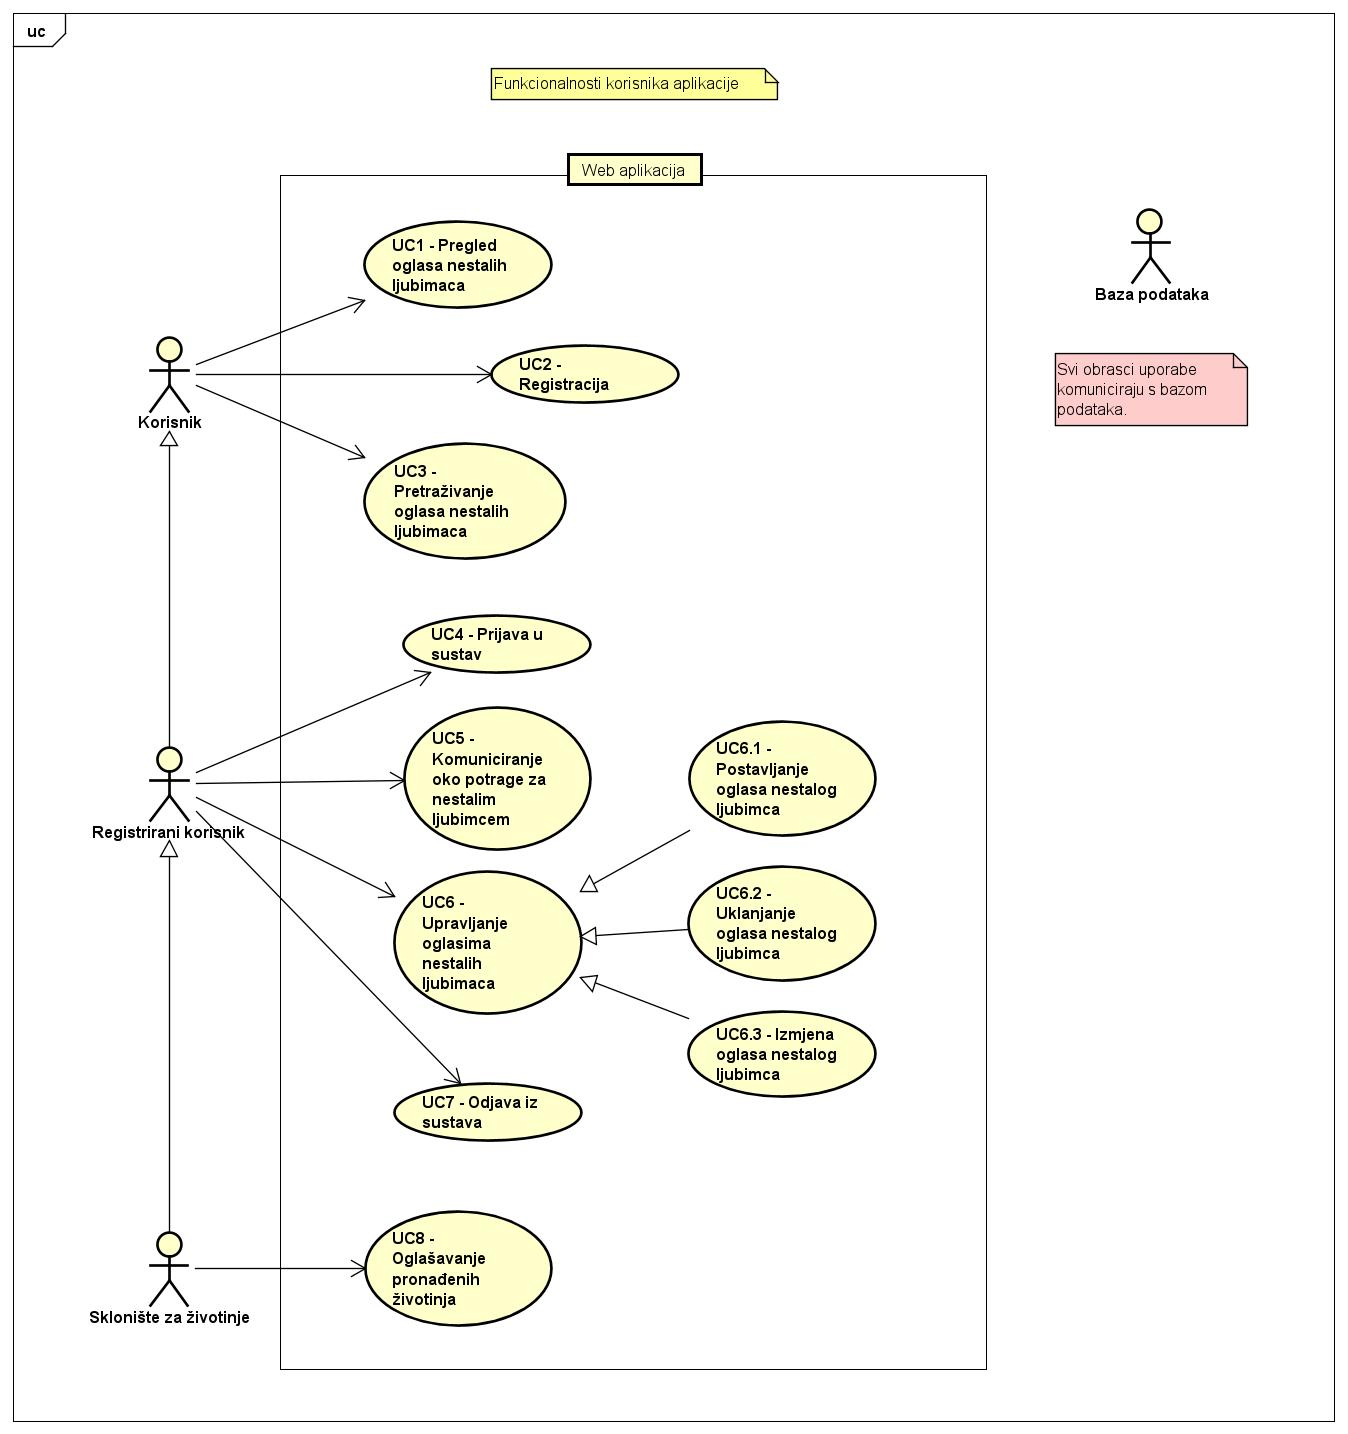
\includegraphics[width=\textwidth]{slike/funkcionalnost_korisnika.jpg}
						\caption{Dijagram obrasca uporabe, funkcionalnost korisnika}
					\end{figure}		
				
			\pagebreak
			\subsection{Sekvencijski dijagrami}

				\begin{figure}[hp!]
					\centering
					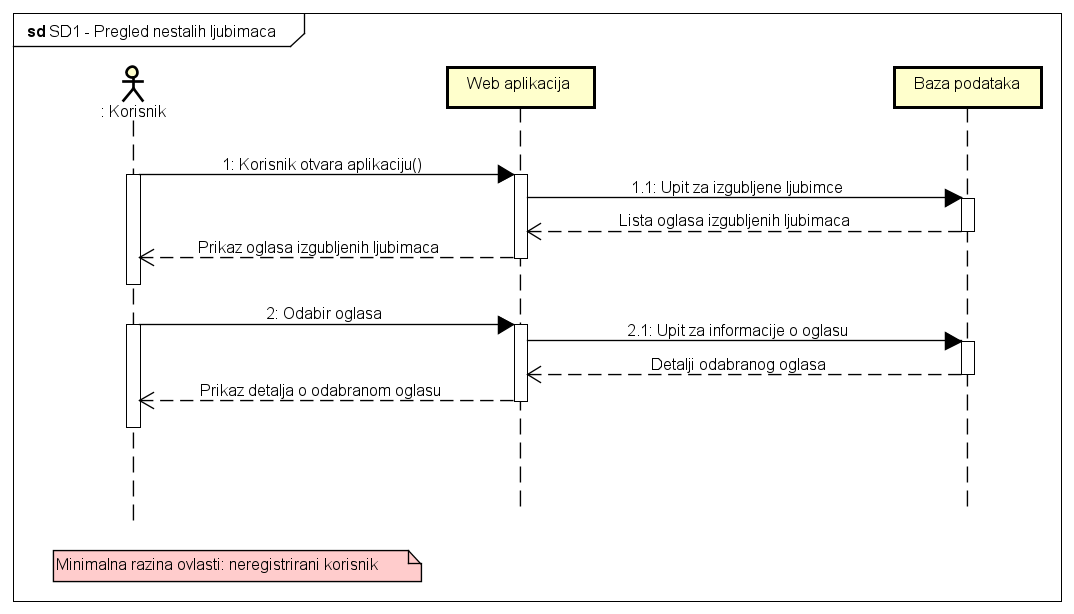
\includegraphics[width=\textwidth]{slike/SD1 - Pregled nestalih ljubimaca.png}
					\caption{Sekvencijski dijagram - Pregled nestalih ljubimaca}
					\begin{flushleft}
						\textbf{Detaljnije objašnjenje:}
						Nakon što korisnik otvori aplikaciju, aplikacija će poslati upit bazi podataka za trenutno aktivne oglase. Odgovor baze se zatim formira u obliku popisa oglasa koji se prikazuju korisniku. Nakon što korisnik odabere oglas, aplikacija šalje upit bazi podataka za detaljnim informacijama o odabranom oglasu. Baza podataka vraća detaljne informacije o odabranom oglasu. Aplikacija zatim prikazuje detaljne informacije o odabranom oglasu i moguće metode komunikacije.
					\end{flushleft}
				\end{figure}
				\pagebreak
				\begin{figure}[hp!]
					\centering
					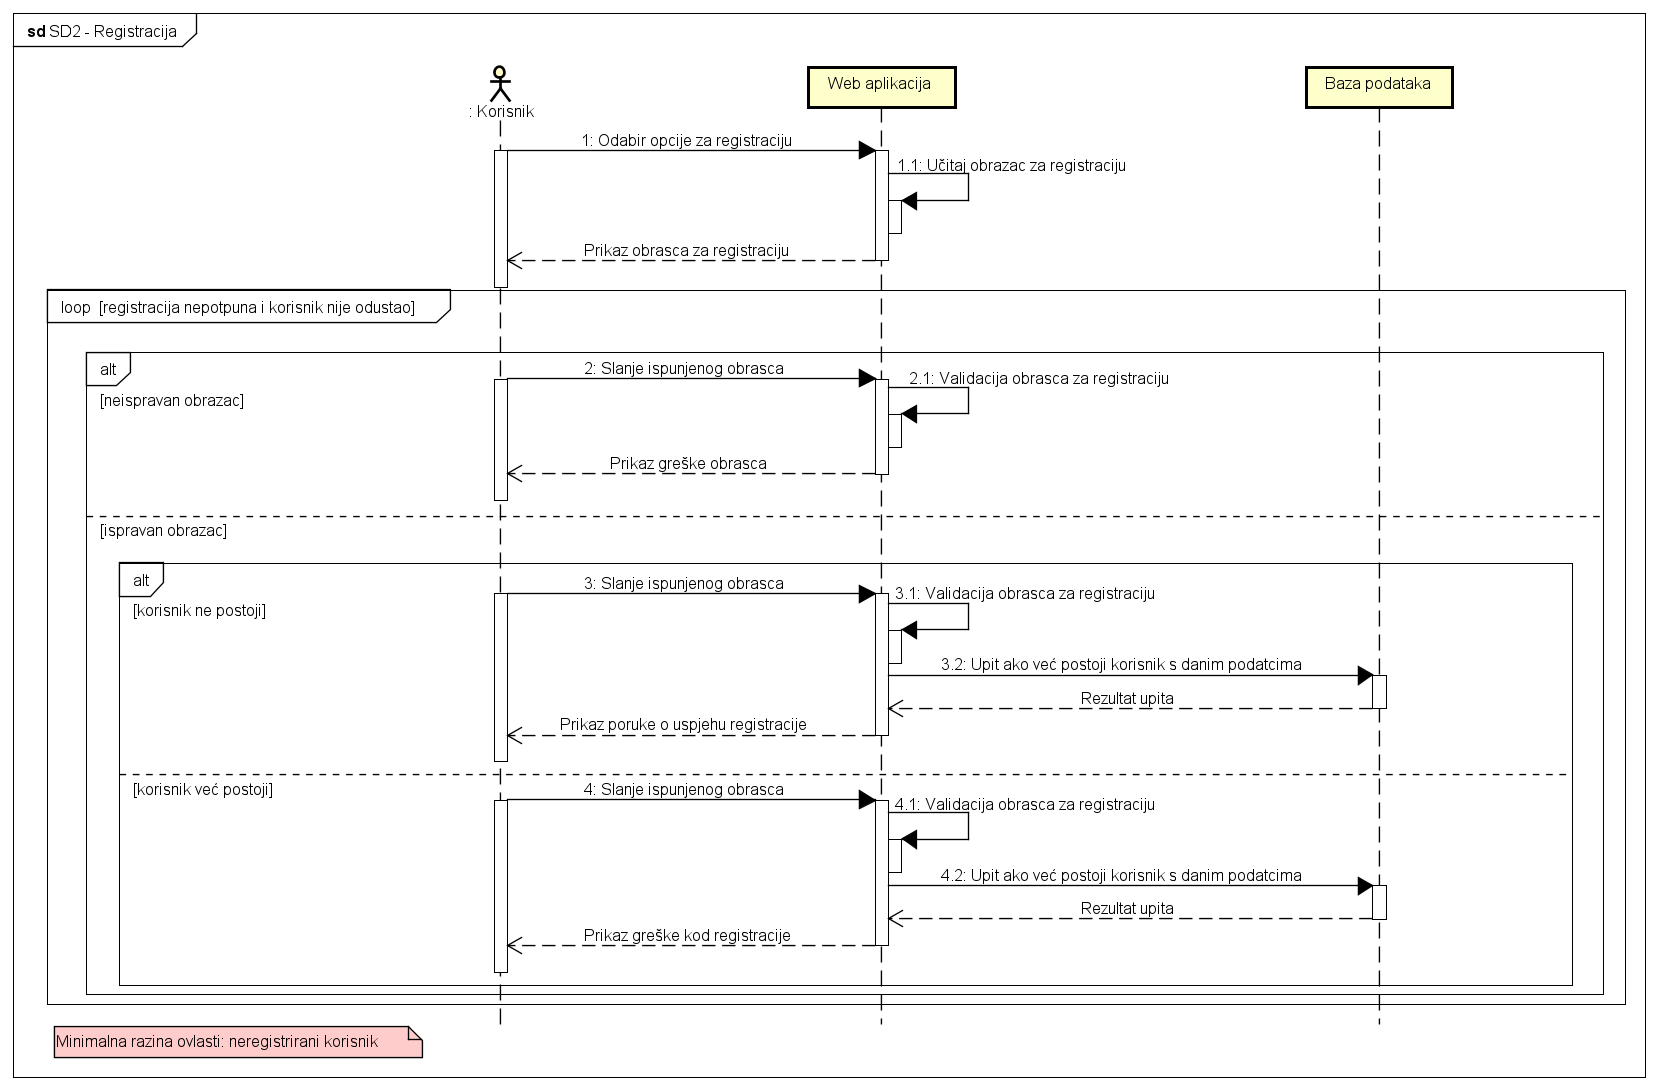
\includegraphics[width=\textwidth]{slike/SD2 - Registracija.png}
					\caption{Sekvencijski dijagram - Registracija}
					\begin{flushleft}
						\textbf{Detaljnije objašnjenje:}
						Nakon što korisnik odabere opciju registracije, aplikacija učitava obrazac i prikazuje ga korisniku. Korisnik zatim ispunjava i šalje ispunjen obrazac nad kojim se provodi validacija (provjera jesu li ispravno ispunjena potrebna polja), a zatim upit prema bazi podataka ako korisnik s danim podatcima već postoji. Ako korisnik s danim podatcima ne postoji, aplikacija šalje upit bazi podataka za spremanje novog korisnika. Baza podataka zatim sprema novog korisnika i vraća odgovor aplikaciji. Aplikacija zatim prikazuje poruku o uspješnoj registraciji. U suprotnom, aplikacija prikazuje odgovarajuću poruku (korisnik već postoji ili obrazac nije ispravno popunjen). Proces ispunjavanja obrasca se odvija sve dok korisnik ne odustane od registracije ili ne uspije uspješno provesti registraciju.
					\end{flushleft}
				\end{figure}
				\pagebreak
				\begin{figure}[hp!]
					\centering
					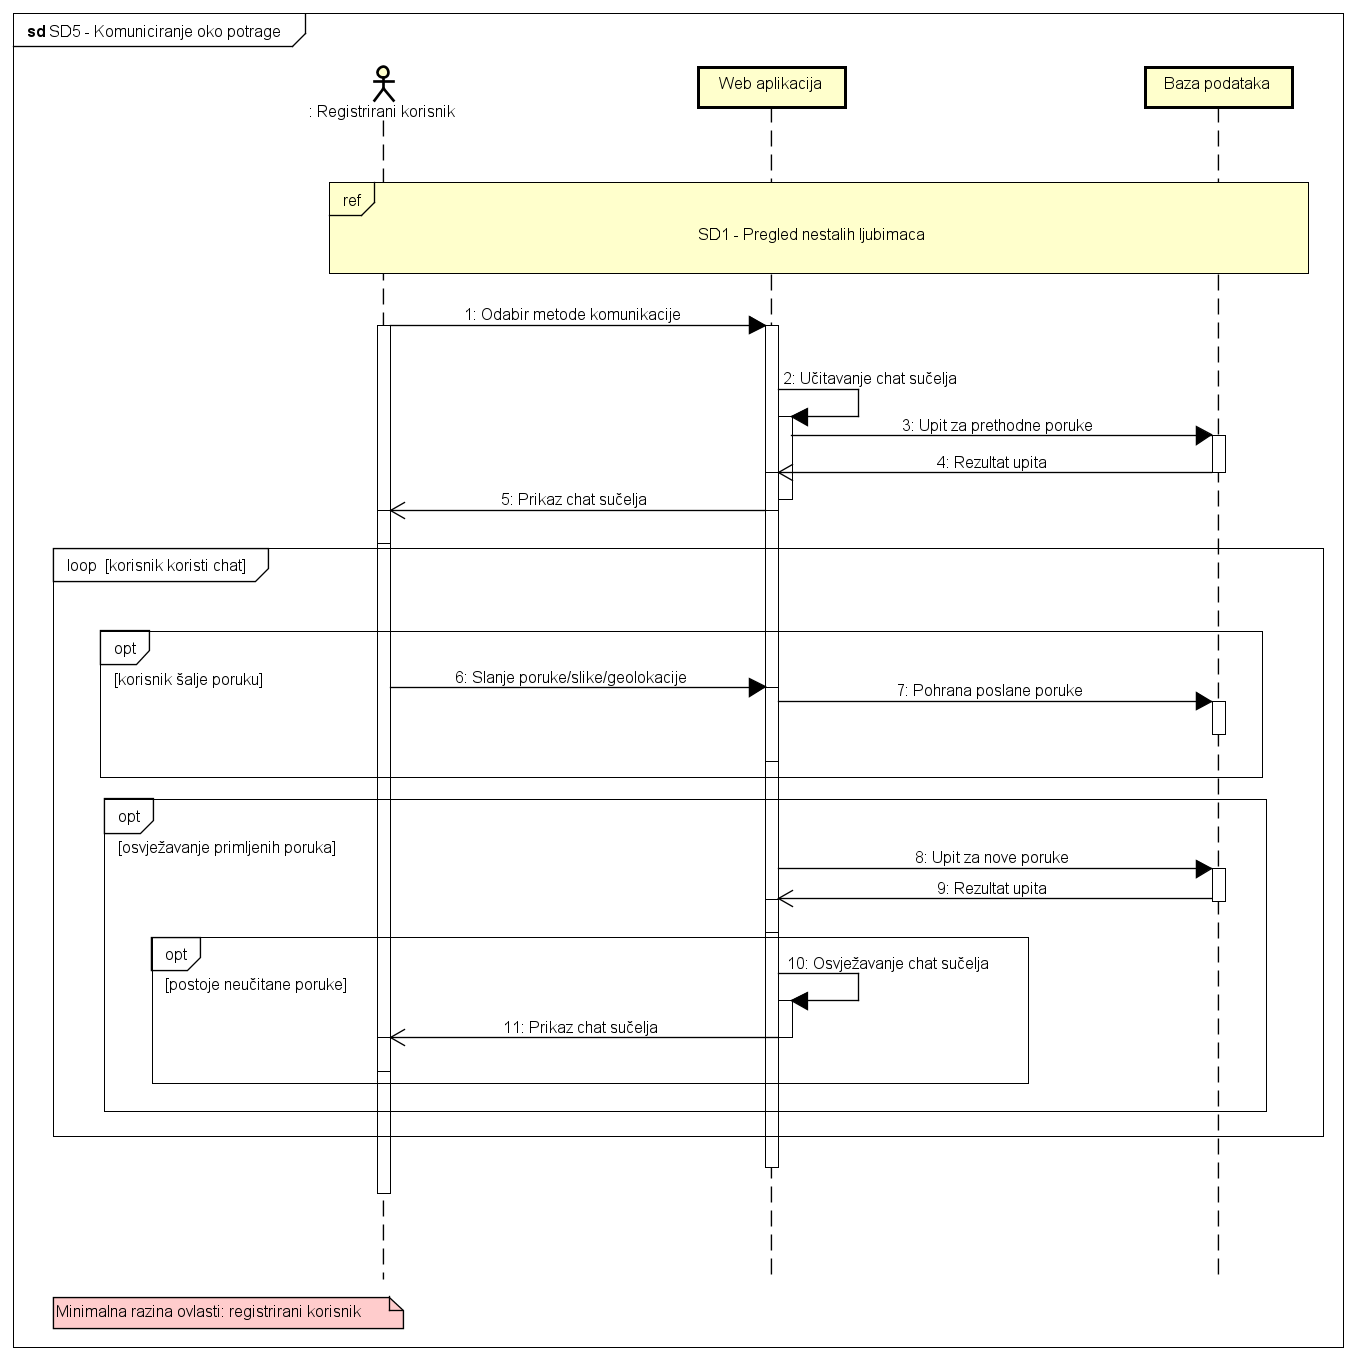
\includegraphics[width=\textwidth]{slike/SD5 - Komuniciranje oko potrage.png}
					\caption{Sekvencijski dijagram - Komuniciranje oko potrage}
					\begin{flushleft}
						\textbf{Detaljnije objašnjenje:}
						Korisnik odabere oglas i opciju komunikacije. Aplikacija učita chat sučelje i šalje upit bazi podataka za sve prethodne poruke. Baza podataka vraća prethodne poruke koje aplikacija prikazuje korisniku. Korisnik unese poruku i aplikacija je šalje bazi podataka. Baza podataka sprema poruku i vraća odgovor aplikaciji. Aplikacija prikazuje poruku korisniku. U određenim intervalima, aplikacija šalje upit bazi podataka za nove poruke. Baza podataka vraća nove poruke koje aplikacija prikazuje korisniku. Proces se nastavlja dok korisnik ne napusti chat sučelje.
					\end{flushleft}
				\end{figure}
				\pagebreak
				\begin{figure}[hp!]
					\centering
					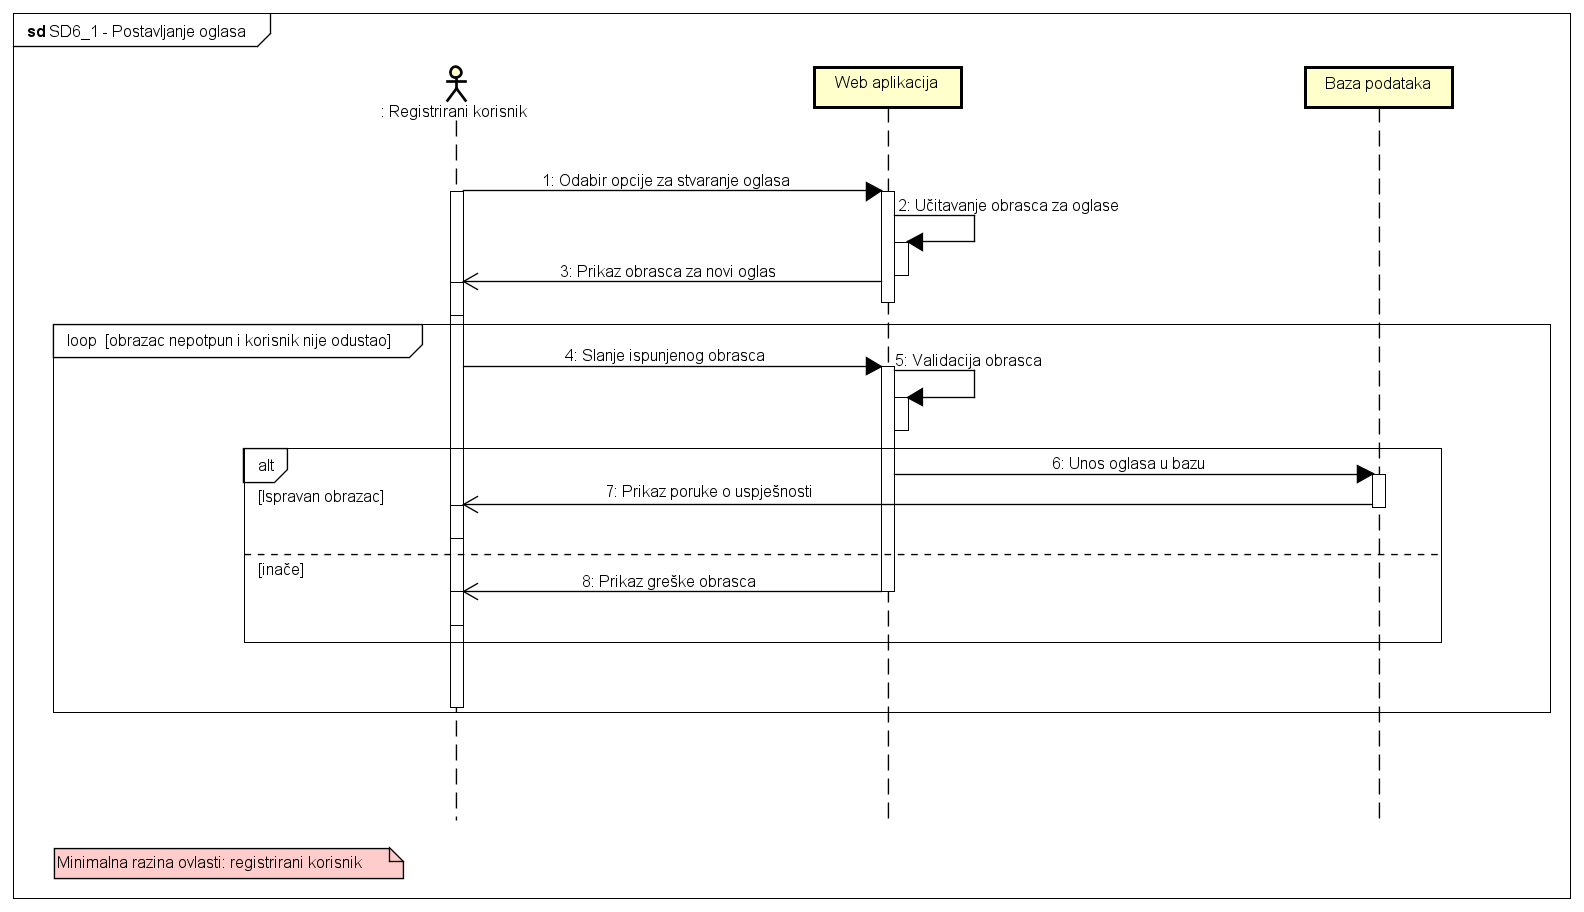
\includegraphics[width=\textwidth]{slike/SD6_1 - Postavljanje oglasa.png}
					\caption{Sekvencijski dijagram - Postavljanje oglasa}
					\begin{flushleft}
						\textbf{Detaljnije objašnjenje:}
						Korisnik odabere opciju za novi oglas. Aplikacija učitava obrazac i prikazuje ga korisniku. Korisnik zatim ispunjava i šalje ispunjen obrazac nad kojim se provodi validacija (provjera jesu li ispravno ispunjena potrebna polja). Ako je obrazac ispravno ispunjen, aplikacija šalje upit bazi podataka za spremanje novog oglasa. Baza podataka zatim sprema novi oglas i vraća odgovor aplikaciji. Aplikacija zatim prikazuje poruku o uspješnoj objavi oglasa. U suprotnom, aplikacija prikazuje odgovarajuću poruku (obrazac nije ispravno popunjen). Proces ispunjavanja obrasca se odvija sve dok korisnik ne odustane od objave oglasa ili ne uspije uspješno objaviti oglas. 
					\end{flushleft}
				\end{figure}
				\eject

		\section{Ostali zahtjevi}

            \begin{itemize}
                \item Osnovni jezik korisničkog sučelja je hrvatski.
                \item Sustav treba podržati hrvatski jezik i hrvatske dijakritičke znakove - Unicode standard .
                \item Vrijeme odgovora na korisnički zahtjev ne smije biti duže od nekoliko sekundi, mora biti prikladno hitnosti zahtjeva.
                \item Sustav mora podržati rad više korisnika istovremeno.
                \item Sustav mora biti jednostavan i korisničko sučelje intuitivno za korištenje.
                \item Web aplikacija mora biti responzivna, potrebno je uzeti u obzir korisnike koji pristupaju putem mobilnih uređaja, tableta i sl.
                \item Komunikacija između korisnika i poslužitelja mora biti kriptirana, potrebno implementirati SSL vezu odnosno HTTPS protokol.
                \item Iznenadni prekid rada sustava ne smije ugroziti unesene podatke korisnika.
                \item Neispravno korištenje korisničkog sučelja ne smije narušiti funkcionalnost sustava.

            \end{itemize}			 
	